% This must be in the first 5 lines to tell arXiv to use pdfLaTeX, which is strongly recommended.
\pdfoutput=1
% In particular, the hyperref package requires pdfLaTeX to break URLs across lines.

\documentclass[11pt]{article}

% Remove the "review" option to generate the final version.
\usepackage[]{NLPAICS2024}

% Standard package includes
\usepackage{times}
\usepackage{graphicx} % Required for inserting images
\usepackage{amssymb}

\usepackage{latexsym}
\usepackage{indentfirst}
% For proper rendering and hyphenation of words containing Latin characters (including in bib files)
\usepackage[T1]{fontenc}
% For Vietnamese characters
% \usepackage[T5]{fontenc}
% See https://www.latex-project.org/help/documentation/encguide.pdf for other character sets

% This assumes your files are encoded as UTF8
\usepackage[utf8]{inputenc}

% This is not strictly necessary, and may be commented out.
% However, it will improve the layout of the manuscript,
% and will typically save some space.
\usepackage{microtype}

% This is also not strictly necessary, and may be commented out.
% However, it will improve the aesthetics of text in
% the typewriter font.
\usepackage{inconsolata}

\usepackage{fancyhdr}
\pagestyle{fancy}
\usepackage{lastpage} % for \pageref{LastPage}

\fancyhf{} % Clear all header and footer fields
\lhead{14:332:493 Machine Learning for IoT}
\chead{Abid Azad and Ravi Raghavan}
\rhead{Page \textbf{\thepage{}} of \textbf{\pageref{LastPage}}}



% If the title and author information does not fit in the area allocated, uncomment the following
%
%\setlength\titlebox{<dim>}
%
% and set <dim> to something 5cm or larger.

\title{Human-Activity-Recognition}

% Author information can be set in various styles:
% For several authors from the same institution:
% \author{Author 1 \and ... \and Author n \\
%         Address line \\ ... \\ Address line}
% if the names do not fit well on one line use
%         Author 1 \\ {\bf Author 2} \\ ... \\ {\bf Author n} \\
% For authors from different institutions:
% \author{Author 1 \\ Address line \\  ... \\ Address line
%         \And  ... \And
%         Author n \\ Address line \\ ... \\ Address line}
% To start a seperate ``row'' of authors use \AND, as in
% \author{Author 1 \\ Address line \\  ... \\ Address line
%         \AND
%         Author 2 \\ Address line \\ ... \\ Address line \And
%         Author 3 \\ Address line \\ ... \\ Address line}

\author{Abid Azad \\
  Rutgers University\\
  \texttt{aa2177@scarletmail.rutgers.edu} \\\And
  Ravi Raghavan \\
  Rutgers University \\
  \texttt{rr1133@scarletmail.rutgers.edu} \\}

\begin{document}
\maketitle

\begin{abstract}
This paper explores the development of machine learning models for Human Activity Recognition (HAR) using smartphone sensor data. The dataset under investigation is sourced from the UCI repository, capturing the movements of 30 individuals engaged in various activities with smartphones strapped to their waists. The study aims to construct predictive models for six human activities, including Walking, Walking Upstairs, Walking Downstairs, Sitting, Standing, and Lying.

Two distinct phases are employed in the approach: the first utilizing classical machine learning algorithms on a pre-engineered dataset, and the second employing deep learning models on raw sensor data. The hypotheses tested include the performance of logistic regression and linear support vector classifier (SVC) as baseline models, the impact of pre-engineered versus raw datasets, the adaptability of transformer and LSTM models, and the influence of training time on model performance.

The experiments reveal that classical models perform well on pre-engineered datasets, while deep learning models show promise with raw sensor data. The LSTM model's accuracy improves with the number of layers, and the transformer model, despite its complexity, lags behind in performance due to data limitations. The study emphasizes the critical role of data preprocessing, model architecture, and dataset characteristics in designing effective HAR systems.

The findings provide valuable insights for researchers and practitioners in tailoring HAR models to real-world scenarios, taking into account the interplay between model complexity and dataset characteristics.
\end{abstract}

\section{Data/System Description}
Smartphones are indispensable tools in our daily lives, enhancing communication and offering intelligent assistance through advanced technology. With a portable device containing computing capabilities and interconnectivity, smartphones provide application programming interfaces for third-party tools and applications. Beyond communication, they boast features like cameras, GPS, and web browsers, along with embedded sensors such as accelerometers and gyroscopes. These sensors enable the development of applications tailored to users' specific location, movement, and context.

One notable application is Activity Recognition (AR), which involves monitoring a person's actions using a smartphone. The widespread use of smartphones has made them a valuable means of identifying environmental changes based on the data collected by built-in sensors. Notably, sensors like the gyroscope and accelerometer contribute to the device's ability to analyze an individual's state.

Human Activity Recognition (HAR) systems leverage raw sensor data collected from smartphones to analyze and interpret human movements. Various deep learning approaches are employed to develop models that accurately identify different human motions.


With the  prospect of deciphering raw sensor data identify human movement, researchers have aggregated datasets that serve as authoritative repositories of information extracted from sensors embedded in smartphones. One particular dataset we are interested in this paper is the Human Activity Recognition (HAR) dataset from the UCI dataset storehouse. In this repository, data from 30 individuals—referred to as subjects—engaged in various activities with smartphones strapped to their waists is meticulously recorded. The sensors, armed with accelerometers and gyroscopes, capture the nuances of their movements. To add a layer of precision, the experiment is thoughtfully video recorded, allowing for manual labeling of the collected data.

Given the density of this particular dataset, the central question guiding this exploration is: Can machine learning models be developed to actively identify and interpret human activity with precision?

\section{Objectives/Hypothesis}
The primary objective of this project is to construct a predictive model for human activities, including Walking, Walking Upstairs, Walking Downstairs, Sitting, Standing, and Lying. Leveraging a relatively modest dataset obtained from the Human Activity Recognition (HAR) Dataset in the UCI repository, our approach involves two distinct phases. The first entails employing a pre-engineered dataset and classical machine learning (ML) algorithms to comprehend and predict human activity. Subsequently, we delve into the raw dataset, utilizing deep learning models to glean insights and forecast human activities.

Human activity recognition poses a formidable challenge, requiring effective time series classification. This task involves predicting an individual's movements based on sensor data, traditionally necessitating profound domain expertise and employing signal processing methods to engineer features from raw data—a prerequisite for fitting a machine learning model accurately.

Ultimately, our project addresses a multiclass classification problem wherein the goal is to predict human activities for a given datapoint, each corresponding to one of the six activities mentioned. To achieve this, we explore the utility of four models. As a foundational step, classical machine learning models such as Logistic Regression and Linear SVC are employed to establish a baseline understanding of the dataset's classifiability using conventional approaches. Subsequently, we aim to enhance the performance benchmarks set by these models by integrating deep learning techniques, specifically Transformers and LSTMs with varying layers.

In formulating our approach, several hypotheses emerge:

\begin{enumerate}

  \item \textbf{Hypothesis on Dataset Impact:}
   \begin{itemize}
      \item The pre-engineered dataset, being tailored for classical ML algorithms, may yield satisfactory results in terms of accuracy.
      \item The raw dataset, with its unprocessed sensor data, may present challenges in feature extraction but holds the promise of capturing more intricate patterns, potentially leading to enhanced performance once processed by deep learning models.
   \end{itemize}

  \item \textbf{Hypothesis on Model Adaptability:}
   \begin{itemize}
      \item Transformers, known for their effectiveness in sequential data tasks, might struggle to demonstrate their full potential within the limited training timeframe and data.
      \item Classical models, being less complex, may adapt more readily to the time constraints, showcasing consistent performance.
   \end{itemize}

\end{enumerate}

Considering these hypotheses, it appears important to conduct a more comprehensive exploration of the dataset, delving into a detailed analysis, and further contemplating strategies for effective data engineering.
\section{Feature Selection and Engineering}

\begin{figure}[h!]
	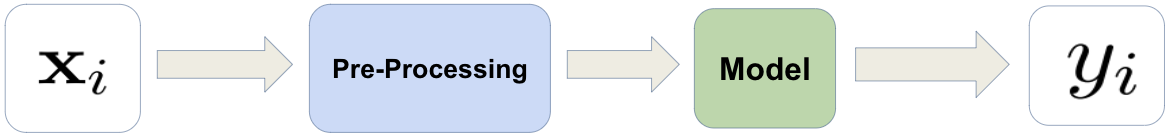
\includegraphics[width= 0.9 \linewidth]{ML Pipeline.png}
	\centering
	\caption{Machine Learning Pipeline}
	\label{ML Pipeline.png}
\end{figure}

As shown by Figure 1, our Machine Learning pipeline resembles a conventional ML Pipeline. First, we receive our input data, which in our case is raw time series data corresponding to accelerometer and gyroscope sensor readings. Then, the aforementioned data is pre-processed and subsequently passed through the Machine Learning Model. Finally, given the output, our system is able to make a prediction regarding the human activity that the data corresponds to. 

In this section, we will be focusing on the Preprocessing Block. We will describe how the preprocessing was done for both the Baseline models and for the Deep Learning Models  

\subsection{Baseline Models}

\begin{figure}[h!]
	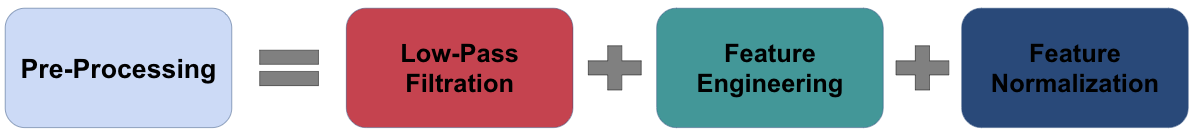
\includegraphics[width= 0.9 \linewidth]{Preprocessing.png}
	\centering
	\caption{Preprocessing}
	\label{Preprocessing.png}
\end{figure}

Figure 2 encapsulates the Preprocessing block used for baseline machine learning models that we used.

\subsubsection{Low Pass Filtration}
This section entails the low pass filtration which essentially used a 1st Order Butterworth low-pass filter to separate accelerometer sensor data into body acceleration and gravitational components. This is a very common signal processing technique. The purpose is to filter out the high-frequency noise and fast variations in the accelerometer signal, leaving behind the slower-changing gravitational component. \newline 

Let us explain the reasoning behind this. Accelerometer data typically includes both the gravitational acceleration and the body acceleration due to motion. The gravitational component is a constant acceleration vector pointing towards the Earth, while the body acceleration varies based on movement. The body acceleration can vary based on the activity that the test subject. \newline 

A low-pass filter allows low-frequency components to pass through while attenuating higher frequencies. In this project, we chose the cutoff Frequency of the Butterworth Low-Pass Filter to be 0.3 Hz. \newline 

The filtered output represents the gravitational acceleration component. To isolate the body component, we can subtract the graviational acceleration signal from the raw accelerometer data. The result will  represent the body acceleration. \newline 

\subsubsection{Feature Engineering}
Once we have isolated the gravitational and body acceleration components, we perform Feature Engineering. \newline 

For feature engineering, we will be estimating statistical properties from the body/total acceleration signals and the gyroscope signals. Here are a few examples of statistical properties that were used:
\begin{itemize}
    \item mean(): Mean value
    \item std(): Standard deviation
    \item mad(): Median absolute deviation 
    \item max(): Largest value in array
    \item min(): Smallest value in array
    \item sma(): Signal magnitude area
    \item energy(): Energy measure. Sum of the squares divided by the number of values. 
    \item iqr(): Interquartile range 
    \item entropy(): Signal entropy
    \item arCoeff(): Autorregresion coefficients with Burg order equal to 4
    \item correlation(): correlation coefficient between two signals
    \item maxInds(): index of the frequency component with largest magnitude
    \item meanFreq(): Weighted average of the frequency components to obtain a mean frequency
    \item skewness(): skewness of the frequency domain signal 
    \item kurtosis(): kurtosis of the frequency domain signal 
    \item bandsEnergy(): Energy of a frequency interval within the 64 bins of the FFT of each window.
    \item angle(): Angle between to vectors.
\end{itemize}

\subsubsection{Feature Normalization}
All features were normalized to be between -1 to 1. 

\subsection{Deep Learning Models}
For the Deep Learning models, we used raw acceleration and gyroscope sensor data as input into the deep learning model. We did not do the Feature Engineering because, as we learned in class, neural networks, especially deep learning models, are capable of learning hierarchical representations from raw data. By providing raw signals, the network can automatically learn relevant features and representations at different levels of abstraction.

\section{Multimodal Data Patterns}
Prior to doing any pre-processing or machine learning work, the first phase of our project was EDA[Exploratory Data Analysis]. 

\begin{figure}[h!]
	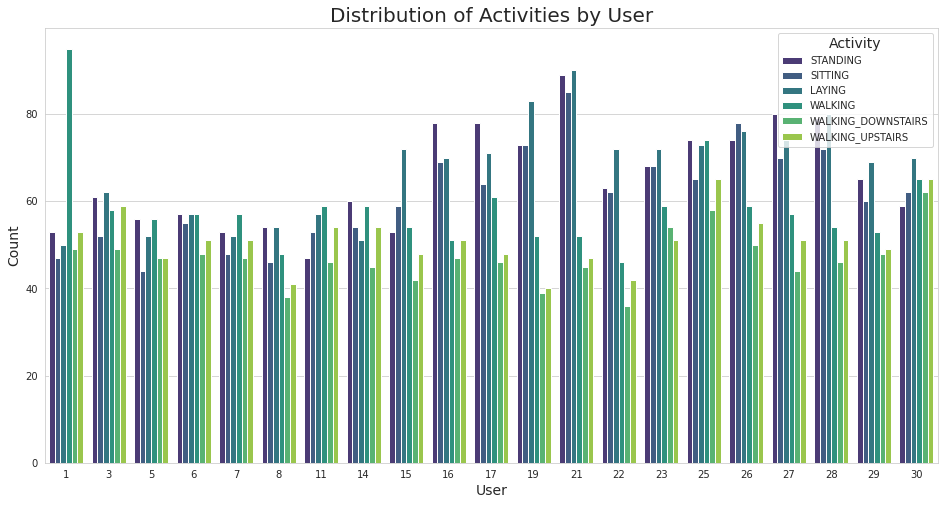
\includegraphics[width= 1.0 \linewidth]{activity_distribution.png}
	\centering
	\caption{Distribution of Activities among Training Experimental Subjects}
	\label{activity_distribution.png}
\end{figure}

Figure 3 shows the distribution of activities among training experimental subjects. The dataset reveals a notable trend wherein participants have a greater volume of data for walking upstairs compared to walking downstairs. Assuming an equal distribution of both uphill and downhill walks, it becomes evident that participants spend a longer duration walking upstairs. \newline 

How is the distribution of activity occurrences in this dataset precisely characterized? Let's generate a plot and delve into the analysis.

\begin{figure}[h!]
	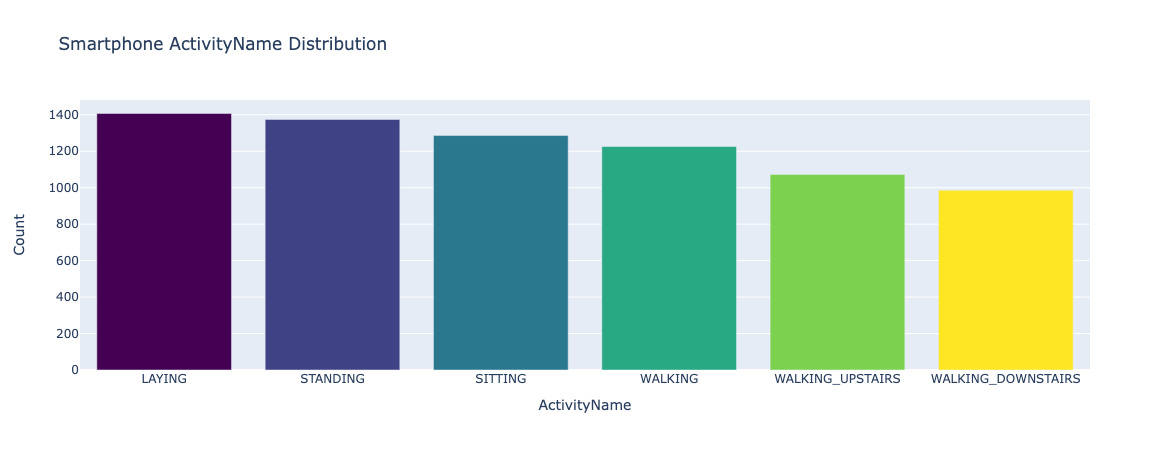
\includegraphics[width= 1.0 \linewidth]{smartphone_activity_name_distribution.png}
	\centering
	\caption{Smartphone Activity Name Distribution}
	\label{smartphone_activity_name_distribution.png}
\end{figure}

Despite fluctuations in label counts, the distribution of labels remains fairly even. Assuming participants ascended and descended an equal number of stairs while smartphones maintained a consistent sampling rate, the dataset should reflect an equal number of data points for both upward and downward walking. Setting aside the potential for flawed data, participants appear to walk approximately 10\% faster when descending. \newline 


Upon initial observation, it is apparent that static activities may not yield as much information as their dynamic counterparts. To substantiate this assertion, let's employ a visual aid for clarification. \newline 

\begin{figure}[h!]
	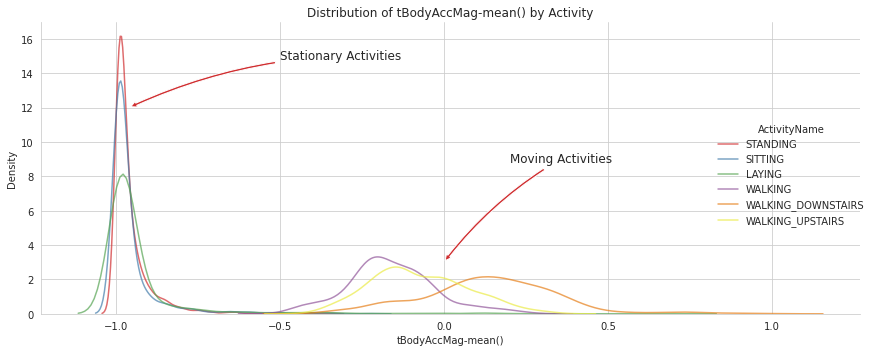
\includegraphics[width= 1.0 \linewidth]{distribution_acc_activity.png}
	\centering
	\caption{Distribution of the Magnitude of Body Acceleration Component}
	\label{distribution_acc_activity.png}
\end{figure}

Explanation of Above Graph: \newline 
\begin{itemize}
    \item The first thing to keep in mind that features in $X\_train.txt$ are normalized and bounded within [-1,1].
    \item Now, let's look at the variable we are analyzing. tBodyAccMag-mean() is the mean magnitude of the body acceleration in the time domain. 
    \item So, at the "-1" end of the graph, this would correspond to a mean magnitude of 0. As we go rightward, this would correspond to an increase in the  mean magnitude of the body acceleration
    \item We can see that, for stationary data, the mean magnitude of body acceleration is roughly 0. This would correspond to expectations
    \item We can see that, for motional data, the mean magnitude of body acceleration is more than 0. This would correspond to expectations. 
\end{itemize}


In real-world datasets, what is often observed is that the distribution of data during participants' movement tends to follow a normal distribution, albeit with some notable long tails. Notably, the magnitude of dynamic activities is significantly higher than that of stationary activities.  \newline 

Now, let's develop a better visual of the distribution of data amidst the activities. \newline 

\begin{figure}[h!]
	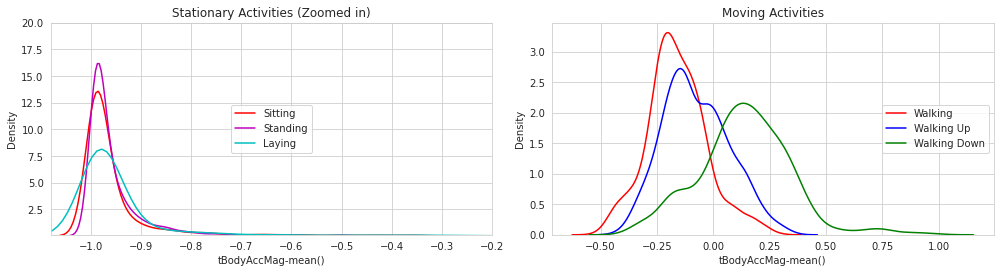
\includegraphics[width= 1.0 \linewidth]{zoomed_distribution_acc_activity.png}
	\centering
	\caption{Zoomed In Distribution of the Magnitude of Body Acceleration Component}
	\label{zoomed_distribution_acc_activity.png}
\end{figure}

The visualizations distinctly illustrate the distribution patterns between Stationary Activities and Moving Activities. Now, the challenge is to precisely differentiate between these activities. One potential approach is to leverage the Magnitude of acceleration as a discriminating factor. To explore this, let's apply a boxplot to visualize and compare the activities.

\begin{figure}[h!]
	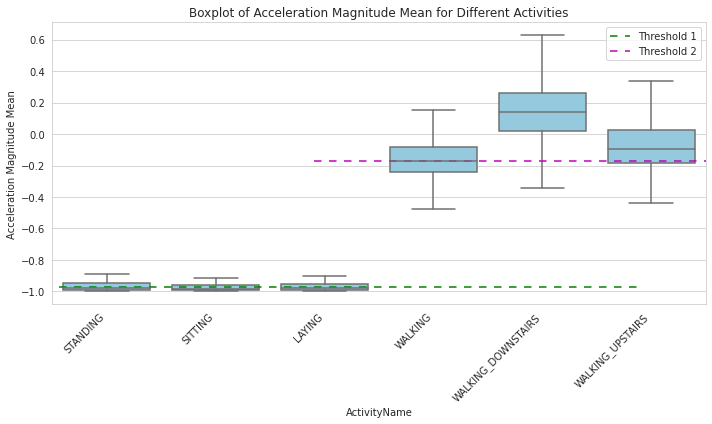
\includegraphics[width= 1.0 \linewidth]{boxplot_acc_magnitude_mean.png}
	\centering
	\caption{Boxplot of Acceleration Magnitude Means}
	\label{boxplot_acc_magnitude_mean.png}
\end{figure}

Analyzing the nuanced patterns unveiled by the box plot reveals valuable distinctions. A tAccMean below -0.8 predominantly corresponds to stationary activities like Standing, Sitting, or Laying. Conversely, when tAccMean exceeds -0.6, it signals dynamic activities such as Walking, Walking Downstairs, or Walking Upstairs. Moreover, a tAccMean surpassing 0.0 specifically characterizes the activity as Walking Downstairs. While achieving a commendable 75\% classification accuracy for activity labels, there remains a margin for error. The consideration of Gravity Acceleration Components adds an additional layer of relevance to the classification task. Thus, revisiting the plots with respect to these components may yield further insights.

\begin{figure}[h!]
	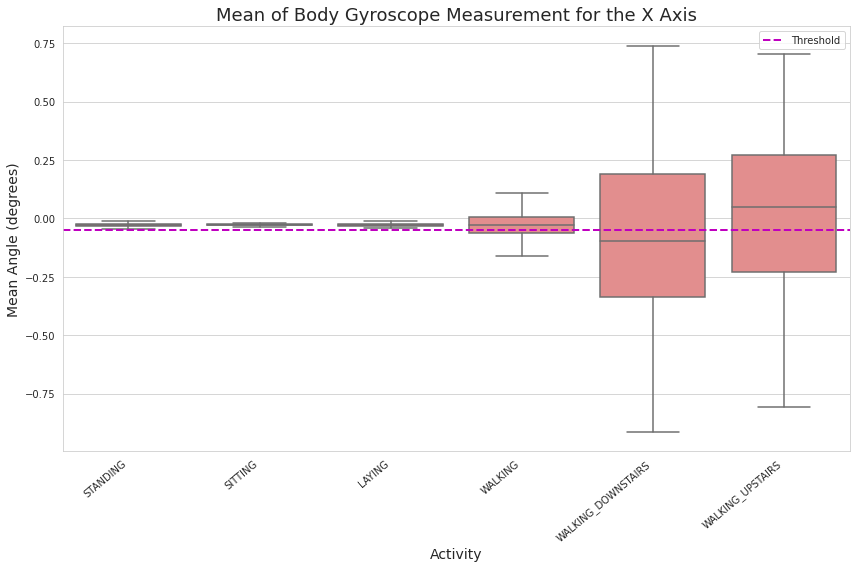
\includegraphics[width= 1.0 \linewidth]{mean_body_gyroscope_x.png}
	\centering
	\caption{Mean of Body Gyroscope Measurement for X Axis}
	\label{mean_body_gyroscope_x.png}
\end{figure}

\begin{figure}[h!]
	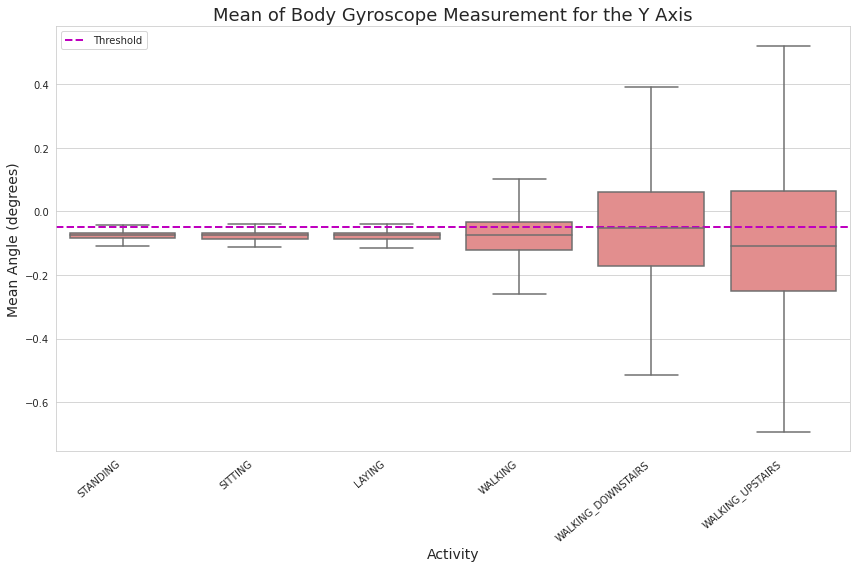
\includegraphics[width= 1.0 \linewidth]{mean_body_gyroscope_y.png}
	\centering
	\caption{Mean of Body Gyroscope Measurement for Y Axis}
	\label{mean_body_gyroscope_y.png}
\end{figure}

\begin{figure}[h!]
	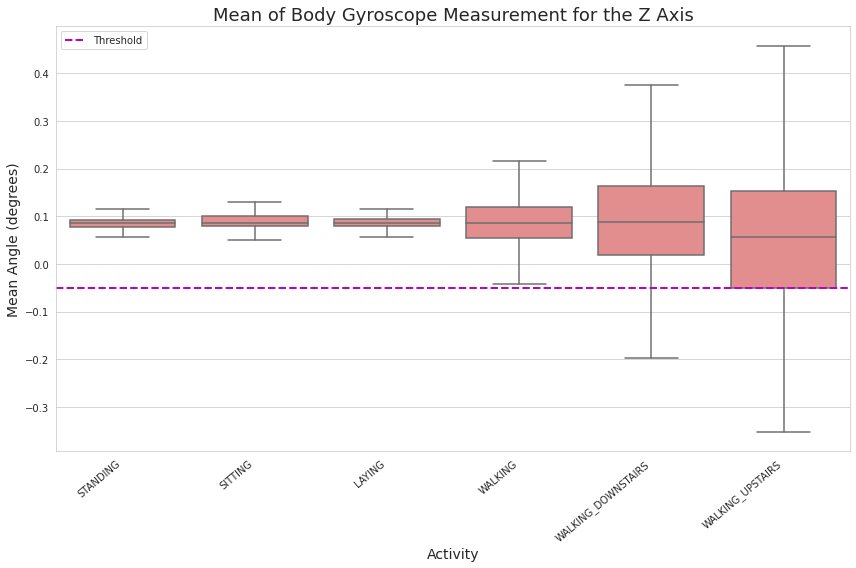
\includegraphics[width= 1.0 \linewidth]{mean_body_gyroscope_z.png}
	\centering
	\caption{Mean of Body Gyroscope Measurement for Z Axis}
	\label{mean_body_gyroscope_z.png}
\end{figure}

The aforementioned gyroscope data clearly shows that there are distinctions in the gyroscope sensor readings among Stationary Activities(i.e. Standing, Sitting, and Laying) versus Motion Activities(i.e. Walking, Walking Upstairs, and Walking Downstairs). This makes perfect sense! Gyroscopes measure angular velocity, which is the rate of rotation. When stationary, the angular velocity is essentially zero, resulting in a relatively stable gyroscope output. This is true because when the gyroscope is stationary, it is affected only by the Earth's gravity. In contrast, when in motion, additional inertial forces come into play, affecting the gyroscope's behavior. Hence, during motion, the gyroscope detects changes in angular velocity, leading to dynamic readings.

\section{Experiments and Methodology}
%Ill fetch the images later.
\textbf{Logistic Regression}: 
Logistic Regression serves as a baseline model, providing insights into the classification task. This linear model, widely employed for binary and multiclass classification, models probabilities using a logistic (sigmoid) function. The logistic function ensures that predictions fall within the range of 0 to 1, making it particularly suitable for classification problems.

We initiated our experiment by fetching and processing data from the Human Activity Recognition (HAR) dataset. Our preprocessing steps involved loading the feature names, training, and testing data. The dataset was divided into singular modality analysis and multimodal analysis, with a subset of features selected for singular modality.

For singular modality analysis, we focused on specific features ('tBodyAcc-mean()-X', 'tBodyAcc-mean()-Y', 'tBodyAcc-mean()-Z') and applied Principal Component Analysis (PCA) to capture 99\% of the variance in the data. \newline 

\underline{Principal Component Analysis}: During our PCA exploration, we started with the original set of engineered features which amounted to 561 features. After conducting PCA, we were able to reduce the number of features to 155. 


The singular modality logistic regression model was then trained on this subset. In the multimodal analysis, the entire set of features was considered. We applied PCA to reduce dimensionality, maintaining 99\% variance. The logistic regression model was trained on this reduced feature set.

To prevent overfitting, we employed L2 regularization (ridge regularization) during the logistic regression model training. Hyperparameter tuning was conducted using grid search with cross-validation to find optimal values for the regularization factor (C) and penalty (l2 or l1).

The trained models were evaluated on the testing dataset, and performance metrics such as accuracy and confusion matrices were computed. Additionally, classification reports were generated to provide a detailed breakdown of the model's performance across different classes.

As a result, the singular modality Logistic Regression model achieved an accuracy of approximately 20.63\% whilst the multimodal Logistic Regression model achieved a significantly higher accuracy of approximately 95.62\%, which , suggests that combining information from a broader set of features, represented by the entire feature set, contributes substantially to the model's ability to accurately classify human activities.


\textbf{Linear SVC}: 
Linear Support Vector Classifier (Linear SVC) serves as a second base line model, offering insights into Human Activity Recognition through classification. Linear SVC aims to find the best-fit hyperplane that separates the data into distinct classes. This hyperplane, once determined, enables the classification of new observations based on their features.

The Linear SVC model follows the same procedure as the Logistic Regression model in terms of setting up the data, creating a singular and multimodal model for analysis, and the reduction of dimensionality through PCA.

Once again, as a reminder \newline 
\underline{Principal Component Analysis}: During our PCA exploration, we started with the original set of engineered features which amounted to 561 features. After conducting PCA, we were able to reduce the number of features to 155. 


The Linear SVC models are then trained on both singular modality and multimodal data. Hyperparameter tuning is conducted using GridSearchCV with cross-validation to find the optimal regularization parameter (C). The tolerance parameter is set to 0.00005 to control the convergence criteria.

As per the other baseline model, trained models are evaluated on the testing dataset, and accuracy metrics are calculated. Additionally, confusion matrices provide insights into the model's performance across different activity classes.

As a result, the singular modality Logistic Regression model achieved an accuracy of approximately 21.99\% whilst the multimodal Logistic Regression model achieved a significantly higher accuracy of approximately 96.20\%, which , suggests that combining information from a broader set of features, represented by the entire feature set, contributes substantially to the model's ability to accurately classify human activities.

\textbf{LSTM:} Based on the nature of this problem, we deemed the LSTM as an integral portion of our system. As we learned in class, Long Short-Term Memory (LSTM) networks are a type of recurrent neural network (RNN) that are well-suited for sequences of data. Since the raw data we have are accelerometer and gyroscope sensor data, this naturally led us towards the LSTM as a key component of our model architecture. Since accelerometer and gyroscope data are inherently sequential data sources, which represent changes in motion over time, we felt that LSTMs would be best to capture dependencies and patterns in our data. 

Additionally, since LSTMs have the ability to capture and retain information over long sequences, we felt that this was very important for understanding complex human activities that dynamically evolve over time.


\begin{figure}[h!]
	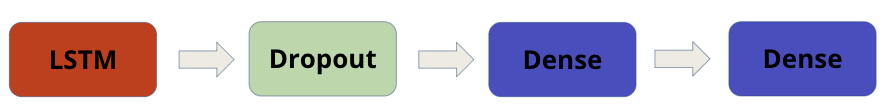
\includegraphics[width= 0.9 \linewidth]{LSTM(1).png}
	\centering
	\caption{LSTM Model Architecture 1}
	\label{LSTM(1).png}
\end{figure}

\begin{figure}[h!]
	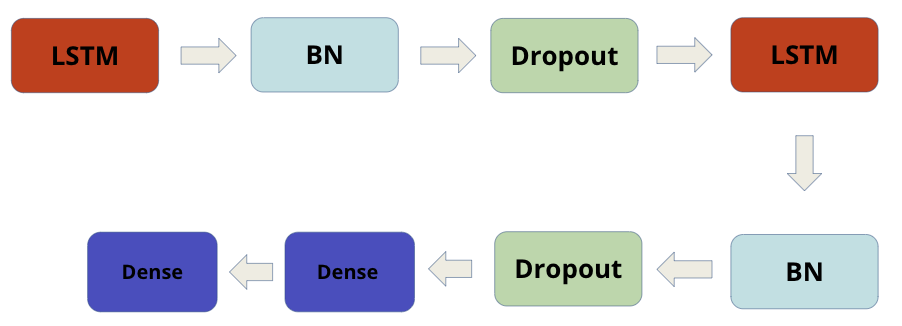
\includegraphics[width= 0.9 \linewidth]{LSTM(2).png}
	\centering
	\caption{LSTM Model Architecture 2}
	\label{LSTM(2).png}
\end{figure}


\begin{figure}[h!]
	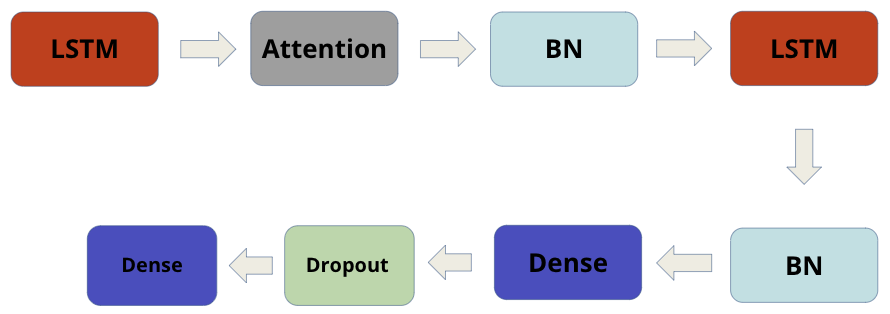
\includegraphics[width= 0.9 \linewidth]{LSTM(3).png}
	\centering
	\caption{LSTM Model Architecture 3}
	\label{LSTM(3).png}
\end{figure}

Here are the three LSTM Model Architectures that we experimented with. Let us dive into each LSTM Model Architecture. 
\subsection{LSTM Model Architecture 1}
This is the first LSTM Model Architecture that we experimented with. Given the input data, the LSTM Layer returned an output vector of size 32. \newline 

Then, we used a Dropout Layer where 50 percent of the inputs were dropped. Finally, we had two Dense Layers at the end. The first Dense layer outputs a vector of size 16. The activation function for this Dense Layer is ReLU \newline 

The second Dense layer outputs a vector of size 6. The activation function for this Dense is softmax \newline 

\begin{figure}[h!]
	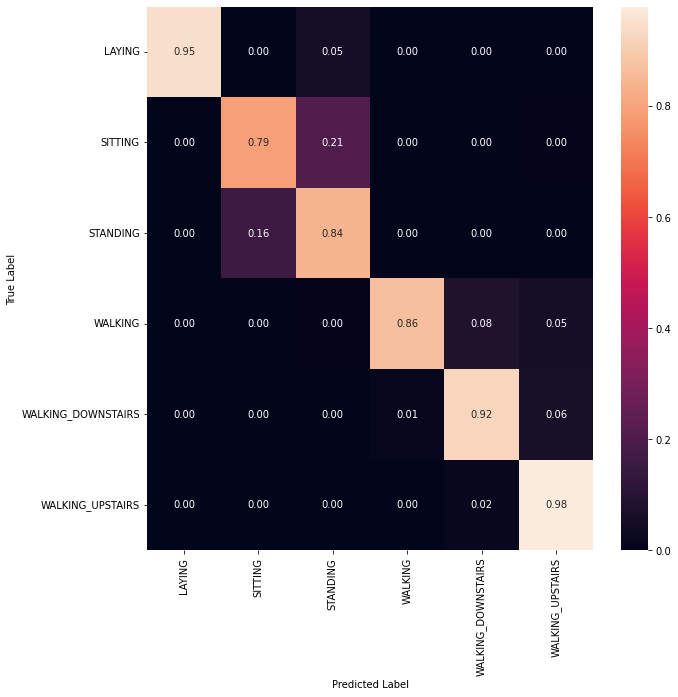
\includegraphics[width= 0.9 \linewidth]{LSTM(1)_Results.png}
	\centering
	\caption{LSTM Model Architecture 1 Results}
	\label{LSTM(1)_Results.png}
\end{figure}

Based on the Confusion Matrix, it is clear that this architecture performs decently well. What we can see is that this model, occasionally, gets mixed up between Standing and Sitting Down. This is quite understandable because when sitting down and standing up, the sensor readings will be roughly the same because both of the aforementioned activities are stationary activities. Hence, to try to get our model to better distinguish between these two activities, we tried two things. The first thing we tried was to increase the number of LSTM Layers. The second thing we tried was to add an Attention Layer to the model. 


\subsection{LSTM Model Architecture 2}
Adding more LSTM layers increases the overall model complexity. Our human activity recognition task requires a more sophisticated representation of temporal dependencies. Hence, having additional LSTM layers may help the model capture and learn intricate patterns within the data. \newline 

Additionally, we thought to add a Batch Normalization layer whose main idea is to normalizes the input of a layer by subtracting the mean and dividing by the standard deviation of that mini-batch. The normalization is applied independently to each feature (or channel) of the input. \newline 

We felt that the BatchNorm layer would be useful for an LSTM model that takes accelerometer data and gyroscope data as input.

The raw accelerometer and gyroscope data have varying ranges. The BatchNorm layer will help normalize these inputs within each mini-batch during training. Normalizing the inputs ensures that the model is less sensitive to the scale of the input features, which will help to improve convergence and training stability. This will also help to make the loss landscape more uniform due to the fact that the BatchNorm layer has made our features on the same scale. \newline 

Based on the results, Architecture 2 seemed to help the system correctly identify more samples where users were sitting. However, this system performs a bit worsely on samples where users are standing. Hence, this doesn't quite solve the problem. 

\begin{figure}[h!]
	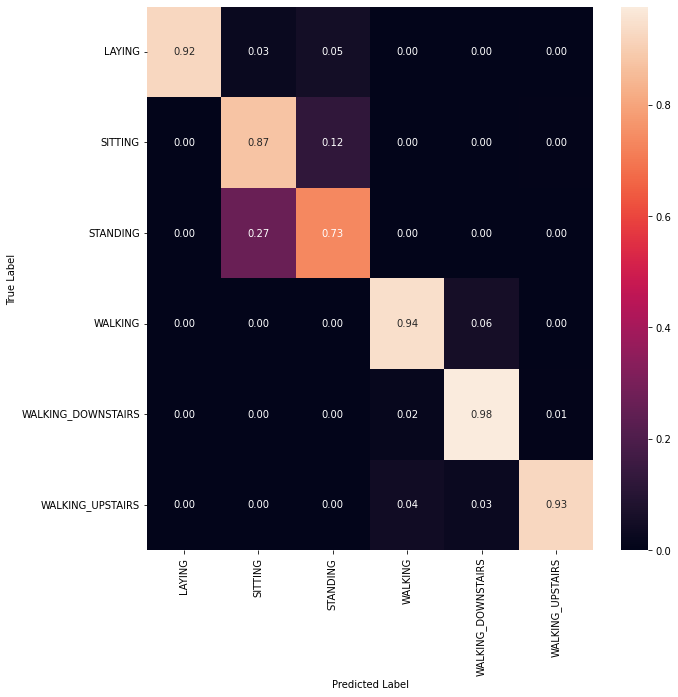
\includegraphics[width= 0.9 \linewidth]{LSTM(2)_Results.png}
	\centering
	\caption{LSTM Model Architecture 2 Results}
	\label{LSTM(2)_Results.png}
\end{figure}

\subsection{LSTM Model Architecture 3}
An important thing to notice about this model architecture is we incorporated an attention layer. As we learned in the course, the purpose of an attention layer in neural networks is to selectively focus on different parts of the input data when making predictions. Instead of treating all input elements equally, the attention mechanism assigns different weights to them, allowing the model to prioritize important information and ignore irrelevant parts. This helps improve the model's ability to capture long-range dependencies and relationships within the input data, making it particularly useful in tasks involving sequential or structured data. \newline 

We believed that incorporating an attention layer within our model architecture would be useful because it would allow the model to focus on specific time steps or intervals, capturing relevant temporal context for recognizing human activities. \newline 

Furthermore, since we have tri-axial accelerometer and gyroscope data, we believed that having an attention layer would enable the model to assign different weights to different sensor readings, emphasizing crucial information and downplaying less relevant data. \newline 

Here is a brief mathematical description of how an Attention Layer works: \newline 

Normally, we would have three sequences be passed into an Attention Layer. We have a Query $Q \in \mathbb{R}^{t \times d}$, a Key $K \in \mathbb{R}^{t \times d}$, and a Value $V \in \mathbb{R}^{t \times d}$. In our case, since we are performing self-attention, $Q = K = V$. \newline 

$Attention(Q, K, V) = softmax(\frac{Q (K^T)}{\sqrt{d}}) V \in \mathbb{R}^{t \times d}$ \newline 

Based on these equations here, it is clear to see that the attention mechanism enables the model to assign different weights to different parts of the input sequence, emphasizing more on the relevant components while downplaying less relevant ones. We felt that this would be particularly useful in time series data where certain time steps may contain critical information for the classification task. \newline 


In our implementation, we extended this concept to implement a Multi-Head Attention Layer. The mathematical concepts behind the Multi-Head attention layer have described, in more detail, in section 5.4. Please refer to that for the more-detailed description! 

Based on the results, Architecture 3 didn't seem to offer much improvement over the Sitting vs Standing Dilemma. Additionally, it seemed to worsen the prediction accuracy for Walking Upstairs Cases. However, for the other categories, it improved the classification accuracy. We believe this occurred because attention mechanisms, especially if the model is complex, can potentially lead to overfitting when the amount of data is limited. Our feeling is that the attention layer we had in this model did not generalize well. 


\begin{figure}[h!]
	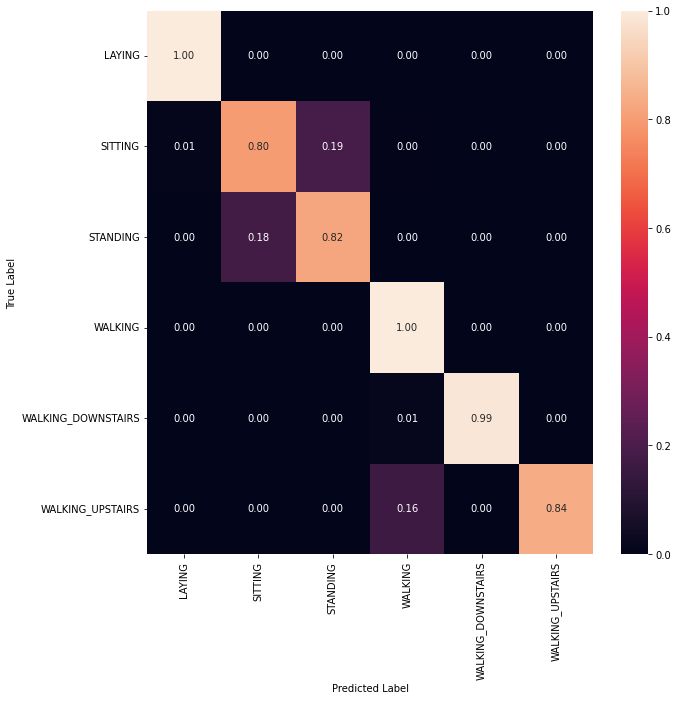
\includegraphics[width= 0.9 \linewidth]{LSTM(3)_Results.png}
	\centering
	\caption{LSTM Model Architecture 3 Results}
	\label{LSTM(3)_Results.png}
\end{figure}

\subsection{Transformer}
Training Multi-Head Attention Layers within the Transformer Model often require a significant amount of data to converge to an optimal solution. In this dataset, we only have 30 subjects and overall roughly 7353 time series samples. Hence, we can say the amount of data is not enough to train the attention layer to converge to an optimal solution. 

\begin{figure}[h!]
	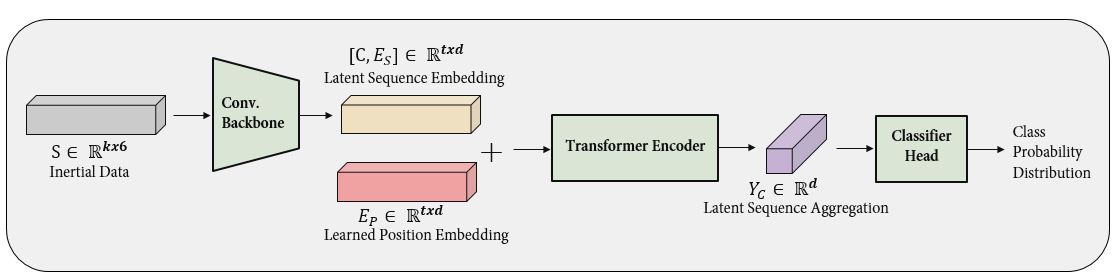
\includegraphics[width= 0.9 \linewidth]{imu_model.png}
	\centering
	\caption{Transformer Model}
	\label{imu_model.png}
\end{figure}

\begin{figure}
    \centering
    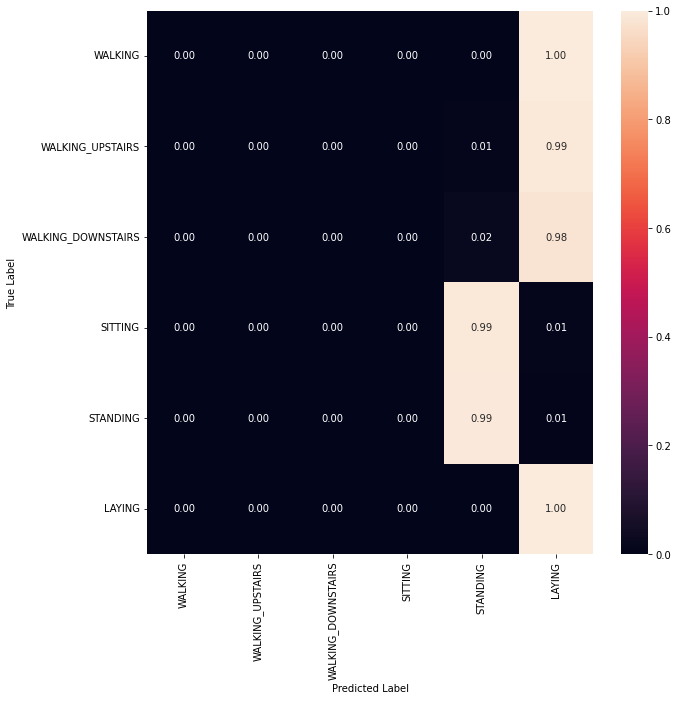
\includegraphics[width= 0.9 \linewidth]{transformer_results.png}
    \caption{Transformer Results}
    \label{transformer_results.png}
\end{figure}

The Transformer Model architecture shown in Figure 17 was an idea taken from Reference [1]. The input is \underline{\textbf{Inertial Data}} which is a matrix of size $\mathbb{R}^{k \times 6}$. In our project case, since we had a total of 9 inertial signals, the input would be of size $\mathbb{R}^{k \times 9}$. \newline 

The next step is to take the Raw Inertial Samples and Embed them in a Higher Dimension. To achieve this, we pass the raw inertial samples through a series of four 1D convolutions that are applied with GELU non-linearity. The end-result of this was to embed the raw data in a higher dimension $d$. Overall, the size of the output of this layer(i.e. $E_S$) should be $\mathbb{R}^{k \times d}$. \newline 

Let $C \in \mathbb{R}^{d}$ represent a class token that is prepended to $E_S$. Additionally, we learn an embedding $E_{P_i} \in \mathbb{R}^d$ for each Position $P_i$ in the sequence $E_S$. 


$Z_0 = [C, E_S] + E_P \in \mathbb{R}^{t \times d}$
where $t = k + 1$ \newline 

We can treat $Z_0$ as the input to the Transformer Encoder. 

\subsubsection{Transformer Encoder}
The Transformer Encoder is comprised of $L$ layers each of which are comprised of a Multi-Head Attention unit followed by a Feedforward Neural Network. \newline 

The Feedforward Neural Network has dimension of $2d$ with GELU Non-linearity. \newline 

\subsubsection{Multi-Head Attention}
Normally, we would have three sequences be passed into a Multi-Head Attention Layer. We have a Query $Q \in \mathbb{R}^{t \times d}$, a Key $K \in \mathbb{R}^{t \times d}$, and a Value $V \in \mathbb{R}^{t \times d}$ \newline 

$h(Q, K, V) = softmax(\frac{Q_h (K_h^T)}{\sqrt{d}}) V_h \in \mathbb{R}^{t \times d'}$ where \newline

$Q_h = QW_h^Q \in \mathbb{R}^{t \times d'}$ \newline 
$K_h = KW_h^K \in \mathbb{R}^{t \times d'}$ \newline 
$V_h = VW_h^V \in \mathbb{R}^{t \times d'}$ \newline 

where $d' = \frac{d}{n_h}$ and $n_h$ represents the number of heads in the Multi-Head Attention Layer \newline 

Evidently, we can treat the matrices $W_h^Q, W_h^K, W_h^V \in \mathbb{R}^{d \times d'}$ as linear projections from the $d$ dimensional space to the $d'$ dimensional space. When we use multi-head attention, we will concatenate the output from each "head" along the channel dimension(i.e. $d$). \newline 

Note: In our case, since we are using self-Multi Head Attention, $Q, K, V$ would all represent the same input sequence! \newline 

To summarize each Transformer Encoder Layer, for $l = 1, 2, 3, ..., L$, we can view it as a two step operation: 
\begin{itemize}
    \item $Z_l ' = sMHA(LN(Z_{l-1})) + Z_{l - 1} \in \mathbb{R}^{t \times d}$
    \item $Z_l = MLP(LN(Z_{l} ')) + Z_{l} ' \in \mathbb{R}^{t \times d}$
\end{itemize}

To get the output of the Transformer Encoder Layer, we take $Y_C = Z_L[0] \in \mathbb{R}^d$ \newline 

\subsubsection{Classification Head}
$Y_C$ is provided as input to the Classification Head. First a Layer Normalization is done. Then, we do a Dense Layer with an output size of $d/4$. Then, we do a GELU Non-Linear Activation. Then, we do a Dropout Layer with 10 percent of the nodes dropped out. Finally, we do a Dense Layer with an output of 6 since we have 6 output classes in our system. 

\section{Conclusion}

\begin{figure}[h!]
    \centering
    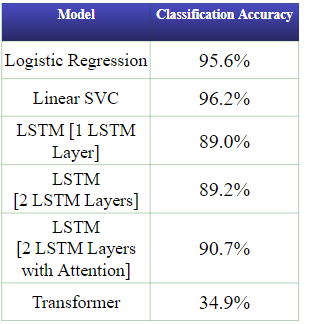
\includegraphics[width= 0.9 \linewidth]{results_IOT.png}
    \caption{Overall Accuracy Results}
    \label{results_IOT.png}
\end{figure}
The unexpected performance of the Transformer model, which demonstrated the lowest accuracy among all models, could be attributed to its intricate architecture and the challenges associated with training attention layers effectively. Transformers are renowned for their success in processing sequential data, especially in natural language tasks. However, their performance can be contingent on the availability of an extensive dataset to train the numerous attention mechanisms effectively. In the context of our HAR dataset, the limited volume of data might have hindered the Transformer's ability to discern and learn the intricate patterns required for accurate activity recognition.

The superior performance of baseline models, such as Logistic Regression and Linear SVC, over Neural Network models raises questions about the interplay between model complexity and dataset characteristics. In scenarios with limited data or simpler underlying patterns, more complex models may struggle to generalize effectively. The baseline models, being less complex and more interpretable, might have exhibited better robustness in the face of these constraints.

The divergence in training processes between Neural Network models and baseline models further emphasizes the importance of data preprocessing. The Neural Network models, specifically LSTM and Transformer, leveraged raw sensor data, with an additional step of decomposing the acceleration data into Body and Gravitational components using low-pass filtration. This preprocessing step was tailored to enhance the model's ability to discern meaningful patterns in the data. On the other hand, the baseline models were trained on preprocessed data, potentially missing out on subtle features present in the raw sensor readings.

The direct correlation observed between the accuracy of the LSTM model and the number of LSTM/Attention Layers emphasizes the importance of model architecture. More complex models, with a greater number of layers, were better equipped to capture intricate temporal dependencies within sequential sensor data. This underscores the need for careful consideration of model architecture based on the nature of the data and the complexity of underlying patterns.

In conclusion, the unexpected findings underscore the nuanced relationship between model complexity, dataset characteristics, and preprocessing steps. The optimal choice of a model for HAR depends on the intricacies of the dataset, and the findings highlight the importance of aligning model selection with the specific requirements and constraints of the task at hand. The analysis provides valuable insights for researchers and practitioners in tailoring HAR systems to real-world scenarios, where data availability and interpretability are crucial considerations.


\section{Reference}\\
Y. Shavit and I. Klein, "Boosting Inertial-Based Human Activity Recognition With Transformers," in IEEE Access, vol. 9, pp. 53540-53547, 2021, doi: 10.1109/ACCESS.2021.3070646.\\\\Messitte, N. (2023, January 6). 6 Ways to Use a Low Pass Filter When Mixing. iZotope. https://www.izotope.com/en/learn/6-ways-to-use-a-low-pass-filter-when-mixing.html\\\\Nafea O, Abdul W, Muhammad G, Alsulaiman M. Sensor-Based Human Activity Recognition with Spatio-Temporal Deep Learning. Sensors. 2021; 21(6):2141. https://doi.org/10.3390/s21062141 

\end{document}
